% !TeX spellcheck = cs_CZ
%{\tikzset{external/prefix={tikz/CES/}}
% \tikzset{external/figure name/.add={ch06_}{}}
%---------------------------------------------------------------------------------------------------
% file CPP.tex
%========================== Kapitola: Přehled jazyka C++============================================
\setchaptertoc
\chapter{Programování v jazyku C++}


  \section{Přehled jazyka C++}\label{CPP:IsecI}
    \texttt{C++} je rozšířená verze jazyka \texttt{C}. \texttt{C++} zahrnuje vše, co je součástí 
    jazyka \texttt{C}, a přidává podporu objektově orientovaného programování (zkráceně 
    \texttt{OOP}). \texttt{C++} navíc obsahuje mnohá vylepšení, a prvky, které z něj jednoduše 
    dělají "lepší \texttt{C}", nezávisle na objektově orientovaném programování. Kromě několika 
    málo zanedbatelných výjimek platí, že \texttt{C} je podmnožinou jazyka \texttt{C++}.

    \luagraphic[0.5]{cpp_fig001.pdf}{C++ je multiparadigmatický programovací jazyk, který vyvinul
    \emph{Bjarne Stroustrup} a další v Bellových laboratořích AT\&T rozšířením jazyka C. C++
    podporuje několik programovacích stylů (paradigmat) jako je \emph{procedurální programování},
    \emph{objektově orientované programování} a \emph{generické programování}, není tedy jazykem
    čistě objektovým. V současné době patří C++ mezi nejrozšířenější programovací jazyky.
    Kredit:Wikipedia}{cpp:fig001} 

    Účelem této kapitoly je představit některé nejdůležitější rysy jazyka C++. Prvky počítačového
    jazyka neexistují izolovaně, vzájemně spolupracují a tvoří úplný programovací jazyk.  Tato
    vzájemnost je obzvláště zřetelná u C++. Lze těžko diskutovat nějaký aspekt jazyka C++ izolovaně
    poněvadž všechny vlastnosti jazyka jsou silně propojeny. Tato kapitola přináší stručný přehled
    některých vlastností C++. Jejich přehled nám umožní porozumnět příkladům, které budou
    diskutovány v následujících kapitolách. 
  
    Poněvadž byl \texttt{C++} vytvořen pro podporu OOP, začne následující podkapitola popisem
    \texttt{OOP}. Jak uvidíme, mnoho prvků jazyka C++ má nějakým způsobem definován vztah k OOP. Je
    důležité si uvědomit, že jazyka \texttt{C++} může byt použito i pro psaní programů, které nejsou
    objektově orientovány. To, jak budemte C++ používat, závisí zcela na nás. 
    
    Tato kapitola, kromě představení nejdůležitějších vlastností jazyka \texttt{C++}, diskutuje
    rozdíly mezi způsoby programování v \texttt{C} a v \texttt{C++}. Existuje několik různých
    přístupů k jazyku C++, která dovolují větší pružnost ve způsobu psaní programů. Přestože některé
    prvky mají jen málo nebo vůbec nic co do činění s \texttt{OOP}, objevují se ve většině programů
    C++ a je vhodné diskutovat je v této knize co nejdříve. \cite[p.~20]{Schildt}.

    \begin{description}[noitemsep]
      \item[C with Classes:] Starší verze jazyka, společně označované jako \uv{C with
        Classes} (česky C s třídami), byly používány od roku 1980. Jméno C++ vymyslel Rick Mascitti
        v létě 1983. Toto jméno zdůrazňuje evoluční povahu změn oproti jazyku C; „++“ je operátor
        inkrementace v C. Kratší jméno „C+“ je syntaktická chyba a bylo též použito jako jméno
        jiného nesouvisejícího jazyka.
      \item[Standardy C++:] Přestože byl jazyk vyvíjen již od počátku 80. let, první oficiální norma
        C++ byla přijata v roce 1998, další v roce 2003 (INCITS/ISO/IEC 14882-2003). V roce 2006 a
        2007 byly přijaty některé aktualizace. Standard označovaný jako C++11, značně rozšířil C++ a
        byl přijat organizací ISO v září 2011 jako ISO/IEC 14882:2011.[1] Současný standard je C++17
        (ISO/IEC 14882:2017).
    \end{description}

    Dříve než začneme, je vhodné uvést několik všeobecných poznámek k povaze a formě jazyka C++.
    Většina součástí programů v jazyce C++ fyzicky vypadá jako programy v jazyce C. Jak programy v
    C, tak i programy v C++ začínají běh v \lstinline[style=luaCPPText]!main()!. Pro zahrnutí
    argumentů příkazového řádku používá C++ tytéž konvence \lstinline[style=luaCPPText]!argc! a
    \lstinline[style=luaCPPText]!argv! jako C. Přestože C++ definuje vlastní objektově orientované
    knihonvy, podporuje rovněž všechny funkce ve standardní knihovně jazyka C. C++ používá stejnou
    řídící strukturu jako jazyk C. C++ zahrnuje všechny zabudované datové typy definované v C. 

    \luagraphic[0.9]{cpp_fig002.jpg}{Bjarne Stroustrup (* 30. prosince 1950, Aarhus, Dánsko) je
    dánský programátor a informatik, profesor na Texas A\&M University a tvůrce programovacího jazyka
    C++.}{cpp:fig002} 

    \subsection{Co je objektově orientované programování (OOP)}
      Objektově orientované programování je výkonný způsob jak přistupovat k úloze programování. Již
      od raných začátků bylo programování spojováno s rozličnými metodologiemi. V každém kritickém
      momentě během vývoje programování byly vytvářeny nové přístupy, které pomohly programátorům
      zvládat stále složitější programy. První programy byly vytvářeny pouhým nastavením přepínačů
      na panelu počítače. Tento postup byl vhodný pouze pro velmi malé programy. Později vytvořený
      jazyk symbolických instrukcí již umožňoval psaní delších programů. K dalšímu vývoji došlo v
      roce 1955, kdy byl vytvořen první programovací jazyk vysoké úrovně - \texttt{FORTRAN}.
    
      S využitím programovacího jazyka vysoké úrovně byl programátor schopen psát programy o délce
      několika tisících řádků. Nejstarší metodou použitou pro programování byl \emph{ad hoc} přístup
      "všechno jde". Jestliže to bylo přípustné pro relativně krátké programy, pak u rozsáhlých
      programů to vedlo k vytváření nečitelných a nezvládnutelných "špagety kódů"
    
      Eliminaci "špagety kódů" umožnil až vznik \emph{strukturovaných programovacích jazyků} v
      šedesátých letech. Byly to jazyky \texttt{Algol} a \texttt{Pascal}. Volně lze interpretovat,
      že je-li jazyk C strukturovaný, pak typ programování, které v něm provádíme, by se mohl
      označit jako strukturované programování. Strukturované programování se opírá o dobře
      definované řídící struktury, bloky kódů, vyloučení příkazů GOTO, lokální (stand-alone)
      podprogramy, které podporují rekurzi, a lokální proměnné. Podstatou struktorovaného
      programování je začlenění programu do jeho základních vymezovacích prvků. S využitím
      strukturovaného programování může průměrný programátor vytvořit a udržovat program o délce až
      \num{50000} řádků. 
    
      Přestože strukturované programování přinášelo výborné výsledky, když bylo použito pro středně
      složité programy, v mnoha bodech zklamalo, když program přesáhl určitou velikost. K tomuto
      účelu bylo vytvořeno objektově orientované programování. OOP vzalo nejlepší myšlenky včleněné
      do strukturovaného programování a zkombinovalo je s výkonnými novými koncepty, které dovolují
      organizovat programy mnohem efektivněji. \texttt{OOP} podněcuje k dekompozici problému na
      základní prvky. Každá komponenta se stává samostatným a nezávislým \textbf{objektem}, který
      obsahuje své vlastní instrukce a data, vztahující se k tomuto objektu. Tímto způsobem je
      komplikovanost snížena a programátor může pracovat s rozsáhlejšímy programy. 
  
      Obecně všechny OOP jazyky sdílejí tři definované vlastnosti:

      \noindent\luafigure[1]{cpp_fig003.pdf}

      \begin{description}[noitemsep]
        \item[\textbf{Zapouzdření}:] je mechanismus, který svazuje dohromady kód a data a
          zabezpečuje je před vnějšími zásahy či před zneužitím. V objektově orientovaném jazyce
          může být kód s daty slučován takovým způsobem, že vznikají jakési nezávislé \uv{černé
          skříňky}. Spojením kódu s daty, vzniká objekt. Jinými slovy lze říci, že objekt je
          instrument, který podporuje zapouzdření.

          Uvnitř objektu může být kód nebo data nebo obojí, jednak jako \emph{privátni} (private)
          vzhledem k objektu, nebo jako \emph{veřejná} (public). Privátní kód nebo data jsou známá a
          dostupná pouze pro jinou část daného objektu. Znamená to, že privátní kód nebo data nejsou
          dosažitelné z jiné části programu mimo objekt. Když jsou kód nebo data veřejná, mohou k
          nim přistupovat i jiné části programu, přestože byly definovány uvnitř objektu. Typicky
          jsou veřejné prvky objektu využity k zajištění řízeného rozhraní k privátním elementům
          objektu.
          
          Pro libovolné účely je objekt proměnná uživatelsky definovaného typu. Může to vypadat
          podivně, že objekt, který spojuje jak kód tak i data, může být považován za proměnnou.
          Ovšem v \texttt{OOP} je tomu přesně tak. Pokaždé, když definujeme nový typ objektu,
          vytváříme nový typ dat. Každý specifický výskyt tohoto typu dat je složená proměnná.

        \item[\textbf{Polymorfismus}:] (z řeckého „mnohotvarost“) je vlastnost, která umožňuje, aby
          bylo jediné jméno použito pro dva nebo více souvisejících, ale technicky různých účelů. Ve
          vztahu k \texttt{OOP} dovoluje polymorfismus určit jedním jménem celou obecnou třídu
          procesů. Uvnitř obecné třídy procesů je pak volba konkrétního procesu dána typem dat. 

          Například v jazyce C, který nijak významně polymorfismus nepodporuje, jsou vyžadována tři
          rozdílná jména pro funkce: \lstinline[style=luaCPPText]!abs()!,
          \lstinline[style=luaCPPText]!labs()! a \lstinline[style=luaCPPText]!fabs()!. Tyto funkce
          vypočítají a vrátí absolutní hodnotu z hodnoty integer, long integer, popřípadě z hodnoty
          s pohyblivou řádovou čárkou. Protože C++ již polymorfismus podporuje, mohou být všechny
          funkce volány pod jediným jménem \lstinline[style=luaCPPText]!abs()!. (Jeden způsob, jakým
          toho lze dosáhnout, je předveden dále v této kapitole.) Typ dat použitý pro volání funkce
          pak určuje, která konkrétní verze funkce bude spuštěna. Jak uvidíme v C++, je možné použít
          jediné jméno funkce pro mnoho různých účelů. Nazývá se to vícenásobná definice funkce.

          Obecně je koncept polymorfismu charakterizován myšlenkou: \uv{jedno rozhraní, mnoho
          metod}, což znamená využití generického rozhraní pro skupiny příbuzných procedur. Výhodou
          polymorfismu je, že omezuje přílišnou složitost tím, že určením \emph{obecné třídy
          procedury} povolí jediné rozhraní. Je pak záležitostí překladače, aby vybral
          \emph{konkrétní proceduru}, vhodnou pro danou situaci. My, programátoři, nemusíme provádět
          tento výběr manuálně. Potřebujeme si pouze zapamatovat a využívat obecné rozhraní. Z
          příkladu v předchozím odstavci je zřejmé, že když pro funkci na určení absolutní hodnoty
          máme místo jediného tři jména, bude se vytvářet obecná procedura pro získání absolutní
          hodnoty podstatně složitěji, než je nezbytně nutné.

          Polymorfismus může být použit také na operátory. Ve skutečnosti všechny programovací
          jazyky obsahují pro aritmetické operátory omezenou aplikaci polymorfismu. Například v
          jazyce C je znaménko + užito k přičítání integer, long integer, znaku nebo hodnoty v
          pohyblivé řádové čárce. Ve všech případech překladač pozná, který typ aritmetiky má
          použít. V C++ můžeme tento koncept dle vlastní definice rozšířit na další typy dat. Tento
          typ polymorfismu se nazývá \emph{vícenásobná definice operátoru}.

          Klíčovým bodem, který si o polymorfismu musíme zapamatovat, je, že dovoluje vytváření
          standardního rozhraní k příslušným procesům.

        \item[\textbf{Dědičnost}:] je proces, při němž může jeden objekt získat vlastnosti jiného
          procesu. Přesněji může objekt zdědit obecnou sadu vlastnosti a do ní může přidat takové
          vlastnosti, které jsou specifické pouze pro něj. Dědičnost je důležitá, protože dovoluje
          objektu podporovat koncept hierarchické klasifikace. Většina informací je vytvářena s
          možností správy hierarchickou klasifikaci. Zkusme se například zamyslet nad popisem domu.
          Dům je částí obecné třídy nazvané budova. Budova je na oplátku zase částí obecnější třídy
          nazvané stavba, kterážto je opět součástí ještě mnohem obecnější třídy objektů zhotovených
          člověkem. V každém případě třída potomka dědí všechny vlastnosti spojené s rodiči a
          přidává k nim své vlastní charakteristiky. Bez využití uspořádané klasifikace by měl každý
          objekt definovány všechny charakteristiky, které se k němu explicitně vztahují.
          Prostřednictvím dědičnosti je však možné objekt udáním obecné třídy (nebo tříd), do které
          patří, aby si zachoval specifické vlastnosti, které jej činí jedinečným. Jak vidíme,
          dědičnost hraje v \texttt{OOP} důležitou roli. 
      \end{description}   
    \subsection{Nové hlavičky C++}
      Povšimněme si dvou řádků v následujícím programu, které jsou bezprostředně za úvodní
      poznámkou. V prvním z nich je přikaz \lstinline[style=luaCPPText]!#include!, kde již není
      \textbf{h} za jménem \lstinline[style=luaCPPText]!iostream!. V následujícím druhém řádku je
      nová specifikace prostoru jmen. Ačkoliv budou moderní hlavičky i prostor jmen detailně
      probrány dále, je nyní na řadě stručný přehled. 
      \begin{lstlisting}[style=luaCPPStyle]
        #include <iostream>
        using namespace std;

        int main()
        {
          /* programovy kod*/
          return 0;
        }
      \end{lstlisting}
      
      Jak víme, v jazyce C se při použití knihonvní funkce musí vložit její hlavičkový soubor.
      Provádí se to příkazem  \lstinline[style=luaCPPText]!#include!. Například v jazyce C vložíme
      pro zahrnutí hlavičkového soubrou I/O funkcí příkaz \lstinline[style=luaCPPText]!stdio.h!
      takto: 
      \begin{lstlisting}[style=luaCPPStyle]
        #include <stdio.h>
      \end{lstlisting}
      Zde je \lstinline[style=luaCPPText]!stdio.h! jménem souboru I/O funkce a použití příkazu
      způsobí, že se tento soubor zahrne do našeho programu. Příkaz
      \lstinline[style=luaCPPText]!#include! způsobí \emph{vložení souboru}.

      Bezprostředně po vytvoření C++ a během několika následujících let byly využívány stejné styly
      hlaviček jako v jazyce C. Standard C++ stále ještě podporuje styly hlaviček jazyka C kvůli
      zpětné kompatibilitě. Standard C++ přinesl nový druh hlaviček, který je ve standardní
      knihovně C++. Nový styl hlaviček nespecifikuje jména souborů. Místo toho se specifikují
      standardní identifikátory, které mohou být mapovány do souborů překladačem, ale také nemusí.
      Nový styl hlaviček je abstrakcí, jež jednoduše zaručuje, že byly deklarovány příslušné
      prototypy a definice požadované knihovnou C++.

      Jelikož nová hlavička není souborem, nemá příponu \textbf{h}. Taková hlavička sestává pouze ze
      jména vloženého mezi lomené závorky. Několik moderních hlaviček, které jsou podporovány
      standardem C++, je uvedeno v následujícím příkladě:
      \begin{lstlisting}[style=luaCPPStyle]
        #include <iostream>
        #include <fstream>
        #include <vector>
        #include <string>
      \end{lstlisting}

      Poněvadž C++ zahrnuje celou knihovnu funkcí jazyka C, podporuje také standardní hlavičky
      jazyka C přidružené k této knihovně. Znamená to, že jsou stále k dispozici hlavičkové soubory
      jako stdio.h a ctype.h. Ovšem standard C++ také definuje nové hlavičky, které můžete použít
      místo starých hlavičkových souborů. V jazyce C++ se ke jménu souboru původní standardní
      hlavičky jazyka C prostě ke přidá předpona \textbf{c} a odejme se \textbf{h}. Nová hlavička
      C++ pro \lstinline[style=luaCPPText]!math.c! je \lstinline[style=luaCPPText]!<cmath>! a
      hlavička pro \lstinline[style=luaCPPText]!string.h! je \lstinline[style=luaCPPText]!cstring!.
      Přestože je přípustné zahrnovat hlavičkové soubory jazyka C, když používáme knihovnu funkcí
      jazyka C, není tento přístup standardem C++ doporučován. 
      
    \subsection{Prostory jmen}
      Když do svého programu vkládáme moderní hlavičku, je obsah této hlavičky obsažen v prostoru
      jmen \lstinline[style=luaCPPText]!std!. Prostor jmen je prostě \emph{deklarativní oblast}.
      Účelem prostoru jmen je lokalizovat jména identifikátorů, a vyhnout se tak kolizím jmen.
      Tradičně byla jména z knihovny funkcí a podobné položky vkládána do globálního prostoru jmen
      (jako je to v jazyce C). Obsah nových hlaviček je umístěn v prostoru jmen
      \lstinline[style=luaCPPText]!std!. Nemusíte z nich mít obavy, protože můžete použít příkaz,
      \begin{lstlisting}[style=luaCPPStyle]
        using namespace std;
      \end{lstlisting}
      který prostor jmen \lstinline[style=luaCPPText]!std! zviditelní (tzn., že přenese
      \lstinline[style=luaCPPText]!std! do globálního prostoru jmen). Jakmile je tento příkaz
      zkompilován, setře se rozdíl mezi prací se starými a novými hlavičkami.
    
    \subsection{Konzola I/O v jazyce C++}
      Protože je C++ rozšířenou množinou jazyka C, jsou všechny prvky jazyka C obsaženy také v C++.
      Z toho vyplývá, že všechny programy C jsou zároveň programy C++. (Ve skutečnosti ovšem
      existují drobné výjimky z tohoto pravidla, které budou diskutovány dále.) Je tedy
      možné psát programy C++ jako programy C. To by samo o sobě nebylo špatné, ale nemohli bychom
      plně využívat všech výhod jazyka C++. Abychom získali maximum z výhod využívání jazyka C++,
      musíme psát nové programy ve stylu C++. To znamená využívat styly kódování a nové prvky, které
      jsou v C++ unikátní.

      Snad nejběžnějším prvkem specifickým pro C++, který je zhusta využíván, je přístup ke konzole
      I/O. Můžeme sice stále ještě využívat funkce jako \lstinline[style=luaCPPText]!printf! a
      \lstinline[style=luaCPPText]!scanf!, ale C++ nám nabízí nový a lepší způsob, jak provádět tyto
      typy I/O operací. V jazyce C++ jsou I/O operace namísto I/O funkcí prováděny pomocí I/O
      operátorů. \textbf{Výstupní operátor} je \lstinline[style=luaCPPText]!<<! a \textbf{vstupní
      operátor} je \lstinline[style=luaCPPText]!>>!. Jak víme, v C slouží tyto operátory jako
      \emph{levý} a \emph{pravý shift}. V jazyce C++ stále ještě přetrvává jejich původní význam
      (levý a pravý shift), ale zároveň přijímají novou rozšířenou roli pro provádění vstupů a
      výstupů. Povšimněme si následujícího příkazu C++:
      \begin{lstlisting}[style=luaCPPStyle]
        cout << "This string is output to the screen. \n";
      \end{lstlisting}
      Tento příkaz způsobí, že se na obrazovce počítače zobrazí řetězec.
      \lstinline[style=luaCPPText]!cout! je předdefinovaný datový proud (stream), který je při
      spuštění programu C++ automaticky připojen ke konzole. Je to podobné jako
      \lstinline[style=luaCPPText]!stdout! v jazyce C. Stejně jako v C může být i v C++ konzola
      přesměrována, ale budeme předpokládat, že je používána. Při použití výstupního operátoru
      \lstinline[style=luaCPPText]!<<! lze provést výstup jakéhokoliv základního typu jazyka C++:
      \begin{lstlisting}[style=luaCPPStyle]
        cout << 100.99;
      \end{lstlisting}
      Obecně platí, že pro výstup na konzolu se používá tato forma operátoru
      \lstinline[style=luaCPPText]!<<!:
      \begin{lstlisting}[style=luaCPPStyle]
        cout << expression; 
      \end{lstlisting}
      Pojmem \emph{výraz} (expression) se míní jakýkoliv platný výraz jazyka C++ včetně dalšího
      výstupního výrazu.

      Pro vstup hodnoty z klávesnice používejme vstupní operátor \lstinline[style=luaCPPText]!>>!.
      Například následující fragment obslouží vstup integer hodnoty do
      \lstinline[style=luaCPPText]!num!.
      \begin{lstlisting}[style=luaCPPStyle]
        int num; 
        cin >> num; 
      \end{lstlisting}
      Povšimněme si, že před \lstinline[style=luaCPPText]!num! není znak
      \lstinline[style=luaCPPText]!&!. Víme, že když pro vstup hodnoty použijeme  \uv{céčkovou}
      funkci \lstinline[style=luaCPPText]!scanf()!, musí funkce nejprve získat adresy proměnných,
      aby ty pak mohly přijmout hodnoty vložené uživatelem. Toto však není nutné, když použijeme
      vstupní operátor C++\footnote{Proč to tak je, se objasní, jakmile se dozvíme víc o C++.}.  
      
      \begin{mdframed}[style=highlight] 
        Rozšířené role operatoru \lstinline[style=luaCPPText]!<<! a
        \lstinline[style=luaCPPText]!>>! je příkladem přetěžování operátoru.
      \end{mdframed}

      Pro používání I/O operátorů v jazyce C++ musíme do programu zařadit hlavičku 
      \lstinline[style=luaCPPText]!<iostream>!. Jak již bylo dříve vysvětleno, je to jedna ze
      standardních hlaviček C++.

      %--iostream-----------------------------------------------------
        % !TeX spellcheck = cs_CZ
\begin{mdframed}[style=mdexam]
  \begin{example}\label{cpp:exam003}
    Výstupem z tohoto programu je řetězec, dvě hodnoty integer a hodnota v rozšířené pohyblivé
    řádové čárce: 
    %---------------------------------------------------------------
      \begin{lstlisting}[style=luaCPPStyle]
        #include <iostream> 
        using namespace std;
        
        int main()
        {
          int i, j; 
          double d;

          i = 10; 
          j = 20; 
          d = 99.101;
          
          cout << "Here are some values: "; 
          cout << i; 
          cout << ' '; 
          cout << j;
          cout << ' '; 
          cout << d;

          return 0;
        }
      \end{lstlisting}
    %---------------------------------------------------------------
    Výstup z programu bude vypadat takto: 
    \begin{mdframed}[style=mdmsdos]
      Here are some values: 10 20 99.101
    \end{mdframed}

    V jediném I/O výrazu je možné provést výstup více než jedné hodnoty. 
      %---------------------------------------------------------------
      \begin{lstlisting}[style=luaCPPStyle]
        cout << i << ' ' << j << ' ' << d;
      \end{lstlisting}
    %---------------------------------------------------------------
    Povšimněme si, že mezi položky musíme explicitně vložit mezery. Když mezera chybí, neoddělená
    data se při zobrazení na obrazovce spojí.
  \end{example}
\end{mdframed}
      %---------------------------------------------------------------

      %--iostream-cin-------------------------------------------------
        % !TeX spellcheck = cs_CZ
\begin{mdframed}[style=mdexam]
  \begin{example}\label{cpp:exam004}
   Tento program vybídne uživatele ke vložení hodnoty integer:
    %---------------------------------------------------------------
      \begin{lstlisting}[style=luaCPPStyle]
        #include <iostream> 
        using namespace std;
        
        int main()
        {
          int i;

          cout << "Enter a value: "; 
          cin >> i;
          cout << "Here's your number: " << i << "\n";

          return 0;
        }
      \end{lstlisting}
    %---------------------------------------------------------------
    Zde je příklad běhu programu:
    \begin{mdframed}[style=mdmsdos]
      Enter a value: 100 \newline
      Here's your number: 100
    \end{mdframed}  
    Hodnota vložená uživatelem je, jak vidíte, předána do \texttt{i}. 

    Program nyní trochu zmodifikujeme tak, aby uživatele vybídla ke vložení hodnoty integer,
    hodnoty v pohyblivé řádové čárce a řetězce. Vše v jediném vstupním příkazu.
    %---------------------------------------------------------------
      \begin{lstlisting}[style=luaCPPStyle]    
        int main()
        {
          int i; 
          float f; 
          char s[80];

          cout << "Enter an integer, float, and string: "; 
          cin >> i >> f >> S; 
          cout << "Here's your data: "; 
          cout << i << ' ' << f «< ' « s;

          return 0;
        }
      \end{lstlisting}
    %---------------------------------------------------------------   
    Tento příklad ilustruje, že v jediném příkazu může vstupovat libovolný počet položek. Stejně
    jako v C musí být položky odděleny vhodnými oddělovacími znaky (mezery, tabelátory nebo konec
    řádku).  

    Při načítání řetězce se vstup zastaví v okamžiku, kdy se objeví první oddělovací znak. Když
    například vložíte do předchozího programu následující data 
    \begin{mdframed}[style=mdmsdos]
      10 100.12 This is a test
    \end{mdframed}  
    zobrazí program toto:
    \begin{mdframed}[style=mdmsdos]
      10 100.12 This
    \end{mdframed}  
    Řetězec není úplný, protože se jeho načítání zastavilo na mezeře za \texttt{This}. Zbytek
    řetězce zůstal ve vstupním bufferu a čeká na další vstupní operaci. (Je to podobné, jako když
    vstupuje řetězec s využitím \lstinline[style=luaCPPText]!scanf()! ve formátu \texttt{\%s}.)   
  \end{example}
\end{mdframed}
      %---------------------------------------------------------------

      Standardně, když použijeme \lstinline[style=luaCPPText]!>>!, jdou všechny vstupy přes
      vyrovnavací paměť. Znamená to, že se do našeho programu C++ nedostane žádná informace, pokud
      nestisknete \texttt{ENTER}. (V jazyce C je funkce \lstinline[style=luaCPPText]!scanf()!
      zpracovávána po řádcích, takže by tento styl práce se vstupem pro nás neměl být nový.) Abychom
      viděli efekt vstupu přes řádkovou vyrovnávací paměť, vyzkoušejme následující program:
      %---------------------------------------------------------------
      \begin{lstlisting}[style=luaCPPStyle]    
        int main()
        {
          char ch;

          cout << "Enter keys, x to stop. \n";
        
          do {
            cout << ": ";
            cin >> ch; 
          } while (ch != 'x');  

          return 0;
        }
      \end{lstlisting}
      %---------------------------------------------------------------  
      Když budeme program zkoušet, budeme muset mačkat \texttt{ENTER} po stisku každé klávesy, aby
      byl vložený znak předán programu.

    \subsection{Třídy: první nahlédnutí}
      Snad nejdůležitějším samostatným prvkem jazyka C++ je \textbf{třída}. Je to mechanismus
      používaný pro vytváření objektů. Jako taková, je třída srdcem mnoha prvků jazyka C++. Třídy
      jsou pro programování v C++ tak významné, že je vhodné předložit na tomto místě jejich stručný
      přehled.
      
      \begin{mdframed}[style=highlight]
        \textbf{Třída} je základním obecným pojmem klasifikace, jak při návrhu uspořádávat informace 
        do smysluplné entity. Základním pojmem je \emph{objekt}, \textbf{instance třídy}, jako 
        konkrétní případ realizace předpisu. Objekt si „pamatuje“ svůj stav (v podobě \textbf{dat} 
        čili \textbf{atributů}) a zveřejněním některých svých operací (nazývaných \textbf{metody}) 
        poskytuje rozhraní, jak s ním pracovat. Při používání objektu nás zajímá, jaké operace 
        (služby) poskytuje, ale ne, jakým způsobem to provádí - to je princip \emph{zapouzdření}. 
        Jestli to provádí sám nebo využije služeb jiných objektů, je celkem jedno. Vlastní 
        implementaci pak můžeme změnit (např. zefektivnit), aniž by se to dotklo všech, kteří 
        objekt používají.
      \end{mdframed}
       
      Abstrakce objektu, která v architektuře programu podchycuje na obecné úrovni podstatu všech
      objektů podobného typu, se nazývá \textbf{třída}. Třída je předpis, jak vyrobit objekt daného
      typu.
  
      Třída je deklarována klíčovým slovem \lstinline[style=luaCPPText]!class!. Syntaxe deklarace
      \lstinline[style=luaCPPText]!class! je podobná její struktuře. V obecné formě vypadá takto
  
      %---------------------------------------------------------------
      \begin{lstlisting}[style=luaCPPStyle]
        class jméno-třídy{
          // privatni-funkce a promenne
        public:
          // verejné funkce a promenne
        } seznam-objektů
      \end{lstlisting}
      %---------------------------------------------------------------
      Seznam objektů je v deklaraci třídy nepovinný. Stejně jako struktura, se  mohou  objekty 
      třídy deklarovat později. Zatímco jméno třídy je také nepovinné, z praktického hlediska je 
      vlastně vždy potřeba. Je to proto, že se jméno třídy stává novým typem jména použitého k 
      deklaraci objektů třídy.
  
      \textbf{Funkce a proměnné} deklarované uvnitř třídy jsou označeny jako \textit{členy této 
      třídy}. Znamená to, že jsou přístupné pouze pro ostatní členy třídy. Pro deklaraci členů 
      veřejné třídy se použije klíčové slovo \lstinline[style=luaCPPText]!public! s dvojtečkou. 
      Všechny funkce a proměn\-né deklarované za tímto specifikátorem jsou přístupné jak pro členy 
      třídy, tak i pro další části programu, které obsahují třídu.
  
      Toto je jednoduchá deklarace třídy:
  
      %---------------------------------------------------------------
      \begin{lstlisting}[style=luaCPPStyle]
        class myclass{
          // privátní vzhledem k myclass
          int a;
        public:
          void set_a(int num);
          int get_a();
        };
      \end{lstlisting}
      %---------------------------------------------------------------
      Tato třída má pouze jednu privátní proměnnou nazvanou \lstinline[style=luaCPPText]!a! a 
      dvě veřejné funkce \lstinline[style=luaCPPText]!set_a()! a 
      \lstinline[style=luaCPPText]!get_a()!. Tyto funkce jsou deklarovány uvnitř třídy pomocí 
      jejich \textbf{prototypů}. Funkce, které jsou deklarovány jako součásti třídy se nazývají 
      \textit{členské funkce}.
  
      Jelikož je \lstinline[style=luaCPPText]!a! privátní, není dostupné pro žádný kód vně
      \lstinline[style=luaCPPText]!myclass!. Ovšem funkce \lstinline[style=luaCPPText]!set_a()! a
      \lstinline[style=luaCPPText]!get_a()! jsou členy \lstinline[style=luaCPPText]!myclass!, takže
      mají k \lstinline[style=luaCPPText]!a! přístup. \lstinline[style=luaCPPText]!set_a()! a
      \lstinline[style=luaCPPText]!get_a()! jsou deklarovány jako veřejné členy
      \lstinline[style=luaCPPText]!myclass! a mohou být volány každou částí programu, která
      \lstinline[style=luaCPPText]!myclass! obsahuje.
  
      Ačkoliv jsou funkce \lstinline[style=luaCPPText]!set_a()! a
      \lstinline[style=luaCPPText]!get_a()!  deklarovány v \lstinline[style=luaCPPText]!myclass!,
      nejsou ještě definovány. Aby jsem definoval členskou funkci, musím spojit typové jméno třídy
      se jménem funkce. To se udělá uvozením jména funkce jménem třídy se dvojicí dvojteček. Dvojice
      dvojteček se nazývá \textit{operátor rozlišení oblasti} (scope resolution operator).
      Následující příklad ukazuje, jak jsou členské funkce \lstinline[style=luaCPPText]!set_a()! a
      \lstinline[style=luaCPPText]!get_a()! definovány:
      %---------------------------------------------------------------
      \begin{lstlisting}[style=luaCPPStyle]
        void myclass::set_a(int num){
          a = num;
        }
    
        int myclass::get_a(){
          return a;
        }
      \end{lstlisting}
      %---------------------------------------------------------------
      Jak \lstinline[style=luaCPPText]!get_a()!, tak i \lstinline[style=luaCPPText]!set_a()! mají
      přístup k \lstinline[style=luaCPPText]!a!, které je privátní v
      \lstinline[style=luaCPPText]!myclass!. Poněvadž \lstinline[style=luaCPPText]!get_a()! i
      \lstinline[style=luaCPPText]!set_a()! jsou členy \lstinline[style=luaCPPText]!myclass!, mohou
      přímo přistupovat k jejím soukromým datům.
  
      Obecně se pro definici členské funkce musí použít následující tvar:
      %---------------------------------------------------------------
      \begin{lstlisting}[style=luaCPPStyle]
        retype jmeno-tridy::jmeno-funkce(seznam-parametru)
        {
        // telo funkce
        }
      \end{lstlisting}
      %---------------------------------------------------------------
      Zde je \texttt{jmeno-tridy} jménem třídy, do níž funkce  náleží.

      Deklarace \lstinline[style=luaCPPText]!myclass! nedefinuje žádný objekt typu
      \lstinline[style=luaCPPText]!myclass!. Definuje pouze typ objektu, který bude vytvořen, když
      bude deklarován. Pro vytvoření objektu se použije jako specifikátor jméno třídy. Například
      tento řádek deklaruje dva objekty typu \lstinline[style=luaCPPText]!myclass!:
      %---------------------------------------------------------------
      \begin{lstlisting}[style=luaCPPStyle]
        myclass ob1, ob2; //toto jsou objekty typu myclass
      \end{lstlisting}
      %---------------------------------------------------------------

      \begin{mdframed}[style=highlight]
        Deklarace třídy je pouze logická abstrakce, jež definuje nový typ. Určuje, jak bude objekt
        daného typu vypadat. Teprve deklarace objektu vytváří fyzickou entitu daného typu. Objekt
        totiž zabírá pamět, ale definiční typ ne.
      \end{mdframed}

      Jakmile je vytvořen objekt třídy, může se program odkazovat na jeho veřejné členy pomocí
      tečkových operátorů bezmála takovým způsobem, jímž jsou prvky struktury zpřístupněny. Dle
      předcházející deklarace objektů volají následující příkazy
      \lstinline[style=luaCPPText]!set_a()! pro objekty \lstinline[style=luaCPPText]!ob1! a
      \lstinline[style=luaCPPText]!ob2!:
      %---------------------------------------------------------------
      \begin{lstlisting}[style=luaCPPStyle]
        ob1.set_a(10); // nastaví verzi ob1 na 10
        ob2.set_a(99); // nastaví verzi ob2 na 99
      \end{lstlisting}
      %---------------------------------------------------------------
      Jak vysvětlují poznámky, tyto příkazy nastavují kopii \lstinline[style=luaCPPText]!ob1! z
      \lstinline[style=luaCPPText]!a! na \lstinline[style=luaCPPText]!10! a kopii
      \lstinline[style=luaCPPText]!ob2! na \lstinline[style=luaCPPText]!99!. Každý objekt obsahuje
      vlastní kopii všech dat deklarovaných uvnitř třídy. Znamená to, že
      \lstinline[style=luaCPPText]!a! náležející \lstinline[style=luaCPPText]!ob1! je odlišné a
      různé od \lstinline[style=luaCPPText]!a! navázaného na \lstinline[style=luaCPPText]!ob2!

      \begin{mdframed}[style=highlight]
        Každý objekt obsahuje vlastní kopii všech dat deklarovaných uvnitř třídy. 
      \end{mdframed}

      %--Nechť má sousedka (chápejme ji jako objekt) má nějaké jméno--
      % !TeX spellcheck = cs_CZ
\begin{mdframed}[style=mdexam]
  \begin{example}\label{cpp:exam002}
    Tento program předvádí \lstinline[basicstyle=\ttfamily]!myclass!, popsanou výše v textu. 
    Nastavuje hodnoty \lstinline[basicstyle=\ttfamily]!a! pro 
    \lstinline[basicstyle=\ttfamily]!ob1! a 
    \lstinline[basicstyle=\ttfamily]!ob2!, a pak zobrazuje hodnotu a pro každý objekt.
    % \marginpar{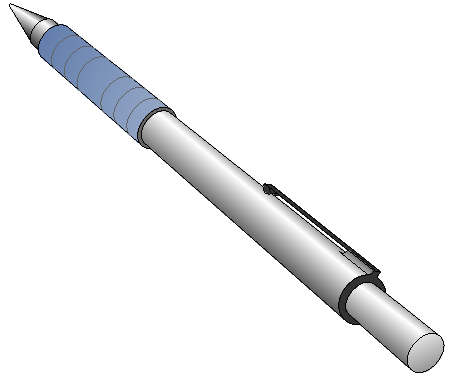
\includegraphics[width=0.05\textwidth]{pen.pdf}}
    \vspace{1em}       
    %---------------------------------------------------------------
    \lstinputlisting[style=luaCPPStyle, caption={\texttt{HS\_37\_myclass.cpp}: představení třídy 
    \texttt{myclass}.}]{../src/CES/CPP/HS_37_myclass.cpp}
    %---------------------------------------------------------------
    Program by měl na obrazovce zobrazit hodnoty \lstinline[basicstyle=\ttfamily]!10! a 
    \lstinline[basicstyle=\ttfamily]!99!.
  \end{example}
\end{mdframed}
      %---------------------------------------------------------------

      V \lstinline[style=luaCPPText]!myclass! z předchozího příkladu je
      \lstinline[style=luaCPPText]!a! privatní. Znamená to, žek ní mohou přímo přistupovat pouze
      členské funkce z \lstinline[style=luaCPPText]!myclass!. (To je důvodem, proč je vyžadována
      veřejná funkce \lstinline[style=luaCPPText]!get_a()!). Jestliže se pokusíme o přístup k
      privátnímu členu třídy z některé části svého programu, který není členem třídy, objeví se při
      překladu chyba. předpokládejme například, že je \lstinline[style=luaCPPText]!myclass!
      definována tak, jak bylo předvedeno v předešlém příkladě. Pak následující volání funkce
      \lstinline[style=luaCPPText]!main()! zapříčiní chybu: 
      %---------------------------------------------------------------
      \begin{lstlisting}[style=luaCPPStyle]
        // Toto je fragment obsahující chybu.
        #include<iostream>
        using namespace std;
        int main()
        {
          myclass ob1, ob2;
          ob1.a = 10; // ERROR! nemuze pristupovat
                      // k privatnimu clenu
          ob2.a = 99; // dle neclenskych funkci.

          cout << ob1.get_a() << "\n";
          cout << ob2.get_a() << "\n";

          return 0;
        }
      \end{lstlisting}
      %---------------------------------------------------------------

      Stejně jako mohou existovat funkce veřejného členu, mohou existovat i proměnné veřejného 
      členu. Jestliže například \lstinline[style=luaCPPText]!a! bylo deklarováno ve veřejné 
      části \lstinline[style=luaCPPText]!myclass!, lze se na ně odkazovat z kterékoliv části 
      programu, jak je předvedeno dále:
      % \marginpar{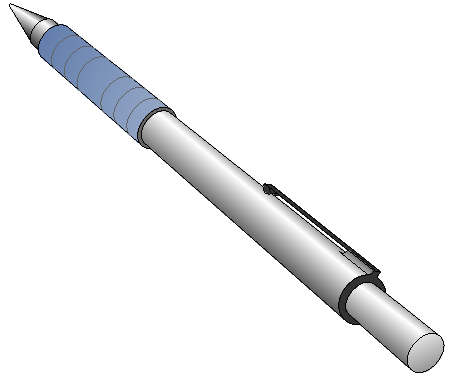
\includegraphics[width=0.09\textwidth]{pen.pdf}}
      %---------------------------------------------------------------
        \begin{lstlisting}[style=luaCPPStyle]
          #include<iostream>
          using namespace std;
  
          class myclass{
          public:
          // nyní je a veřejné
          int a;
          // a  nyní není potřeba set_a() a get_a()
          };
  
          int main()
          {
          myclass ob1, ob2;
  
          ob1.a = 10;
          ob2.a = 99;
  
          cout << ob1.a << "\n";
          cout << ob2.a << "\n";
  
          return 0;
          }
        \end{lstlisting}
      %---------------------------------------------------------------
      Protože je v tomto příkladě \lstinline[style=luaCPPText]!a! deklarováno jako veřejný 
      člen \lstinline[style=luaCPPText]!myclass!, je přímo přístupné z 
      \lstinline[style=luaCPPText]!main()!. Pro přístup k \lstinline[style=luaCPPText]!a! 
      je použit tečkový operátor. Obvykle, když se volá členská funkce nebo se přistupuje k 
      členské proměnné z vnějšího prostředí mimo třídu, je nutná plná specifikace daná jménem 
      objektu i s tečkovým operátorem následovaným jménem člena, aby bylo jasné, na kterého člena 
      objektu se odkazuje.

      Aby byla ukázána síla objektů, následující program \ref{cpp:exam006} vytváří třídu
      pojmenovanou \lstinline[style=luaCPPText]!stack!, která implementuje zásobník použitelný
      například pro uchování znaků:

      %--stack -------------------------------------------------------
      % !TeX spellcheck = cs_CZ
\begin{mdframed}[style=mdexam]
  \begin{example}\label{cpp:exam006}
    Vytvoř třídu \lstinline[style=luaCPPText]!stack!, která implementuje zásobník použitelný pro
    uchování znaků:
    %---------------------------------------------------------------
    \lstinputlisting[style=luaCPPStyle]{../src/CES/CPP/HS_39_stack.cpp}
    %---------------------------------------------------------------
    Program zobrazí následující výstupy:
    \begin{mdframed}[style=mdmsdos]
    Pop s1: c\newline
    Pop s1: b\newline
    Pop s1: a\newline
    Pop s2: z\newline
    Pop s2: y\newline
    Pop s2: x
    \end{mdframed}
  \end{example}
\end{mdframed}
      %---------------------------------------------------------------

      Podívej se na program \ref{cpp:exam006} ještě jednou. Třída
      \lstinline[style=luaCPPText]!stack! obsahuje dvě privátní proměnné:
      \lstinline[style=luaCPPText]!stck! a \lstinline[style=luaCPPText]!tos!. Pole
      \lstinline[style=luaCPPText]!stck! uchovává znaky umístěné v zásobníku a
      \lstinline[style=luaCPPText]!tos! obsahuje index horní úrovně zásobníku. Veřejné funkce
      zásobníku jsou 
      \begin{itemize}[noitemsep]
        \item \lstinline[style=luaCPPText]!init()!,
        \item \lstinline[style=luaCPPText]!push()! a
        \item \lstinline[style=luaCPPText]!pop()!
      \end{itemize}       
      a slouží k inicializaci zásobníku, vkládání hodnoty a k vyjmutí hodnoty. 
      
      Uvnitř funkce \lstinline[style=luaCPPText]!main()! jsou vytvořeny dva zásobníky
      \lstinline[style=luaCPPText]!s1! a \lstinline[style=luaCPPText]!s2! a do každého z nich jsou
      vloženy tři znaky. Je důležité uvědomit si, že každý zásobníkový objekt je oddělený od
      druhého. To znamená, že znaky vložené do \lstinline[style=luaCPPText]!s1! nemohou žádným
      způsobem ovlivnit znaky vložené do \lstinline[style=luaCPPText]!s2!. Každý objekt obsahuje
      vlastní kopii \lstinline[style=luaCPPText]!stck! a \lstinline[style=luaCPPText]!tos!. To je
      základní princip pro pochopení objektů. Ačkoliv všechny objekty třídy sdílejí své členské
      funkce, každý objekt vytváří a udržuje svá vlastní data.
  
    \subsection{Některé rozdíly mezi C a C++}
      Ačkoliv je jazyk C++ rozšířenou množinou jazyka C, existují mezi nimi drobné rozdíly a bylo by
      dobré se s nimi na začátku seznámit. 
      
      Především, když v C nemá funkce žádné parametry, její protyp má v seznamu parametrů funkce
      slovo \lstinline[style=luaCPPText]!void!. Například když v "céčku" funkce nazvaná
      \lstinline[style=luaCPPText]!fl()! nemá parametry (a vrací
      \lstinline[style=luaCPPText]!char!), pak její prototyp bude vypadat následovně:
      %---------------------------------------------------------------
      \begin{lstlisting}[style=luaCPPStyle]
        char fl(void);
      \end{lstlisting}
      %---------------------------------------------------------------
      Přestože v C++ zůstává \lstinline[style=luaCPPText]!void! stále jako volitelný, bude se
      prototyp pro \lstinline[style=luaCPPText]!fl()! psát běžně takto:
      %---------------------------------------------------------------
      \begin{lstlisting}[style=luaCPPStyle]
        char fl();
      \end{lstlisting}
      %---------------------------------------------------------------
  
      C++ se odlišuje od C tím, že je v něm specifikován prázdný seznam parametrů. Kdyby se
      předchozí prototyp objevil v programu C, pak se to bude chápat, že o parametrech nebylo řečeno
      nic. V C++ to znamená, že funkce nemá parametry. Proto tedy v předchozím příkladě nebyl využit
      k deklaraci prázdného seznamu explicitně parametr \lstinline[style=luaCPPText]!void!. (Použití
      parametru void k deklaraci prázdného  seznamu parametrů není zakázáno; je to pouze nadbytečné.
      Jelikož většina programů C++ usiluje o téměř posvátným zanícením o výkonnost,neuvidíme téměř
      nikdy, že by bylo \lstinline[style=luaCPPText]!void! tímto způsobem použito.) Zapamatujme si,
      že v C++ jsou následující dvě deklarace zcela rovnocenné:
      %---------------------------------------------------------------
      \begin{lstlisting}[style=luaCPPStyle]
        char fl();
        char fl(void);
      \end{lstlisting}
      %---------------------------------------------------------------
  
      Další drobná diference mezi C a C++ spočívá v tom, že v programech C++ musí mít všechny 
      funkce prototypy. Zapamatujme si, že v C jsou prototypy doporučeny, ale technicky jsou 
      nepovinné. V C++ jsou však vyžadovány. Jak je patrno z příkladu v předchozí části, prototyp 
      členské funkce obsažený v třídě slouží rovněž jako její obecný prototyp a žádný další 
      samostatný prototyp již není požadován. 
      
      Třetím rozdílem mezi C a C++ je, když je funkce deklarována aby vracela hodnotu, musí hodnotu
      opravdu vracet. Jestliže má totiž funkce jiný návratový typ než
      \lstinline[style=luaCPPText]!void!, musí pak každý příkaz \lstinline[style=luaCPPText]!return!
      uvnitř funkce obsahovat hodnotu. V C není vyžadováno, aby vracely hodnotu funkce, které nejsou
      \lstinline[style=luaCPPText]!void!. Jestliže hodnota neexistuje, "vrací se" jakási nahodilá
      hodnota.
   
      Jestliže v C nespecifikujete explicitně návratový typ funkce, předpokládá se návratový typ
      \lstinline[style=luaCPPText]!integer!. V C++ bylo toto pravidlo potlačeno, a proto musíme
      explicitně deklarovat všechny návratové typy funkcí. Další rozdíl mezi C a C++ je, že v
      programech C budeme muset brát ohled na to, kde mohou být lokální proměnné deklarovány. V C
      mohou být lokální proměnné deklarovány pouze na začátku bloku před všemi "výkonnými" příkazy.
      V C++ mohou být lokální proměnné deklarovány kdekoliv. Výhodou tohoto přístupu je, že lokální
      proměnné mohou být deklarovány tam, kde budou poprvé použity, což může napomoci v prevenci
      před nechtěnými vedlejšími účinky.
  
      Konečně také v C++ definuje datový typ \lstinline[style=luaCPPText]!bool! pro uložení hodnot
      \lstinline[style=luaCPPText]!Boolean! (popř. pravda/nepravda). C++ rovněž definuje klíčová
      slova \lstinline[style=luaCPPText]!true! a \lstinline[style=luaCPPText]!false!, která jsou
      jedinými hodnotami, které může hodnota typu \lstinline[style=luaCPPText]!Boolean! nabývat. V
      C++ je výstupní hodnotou relačních a logických operátorů hodnota typu
      \lstinline[style=luaCPPText]!bool! a všechny podmíněné příkazy musí hodnotu bool vyhodnocovat.
      V C je hodnota \lstinline[style=luaCPPText]!true! nenulová a hodnota
      \lstinline[style=luaCPPText]!false! odpovídá nule. Tak je to i v C++, poněvadž při použití v
      booleánských výrazech je každá nenulová hodnota automaticky převedena na
      \lstinline[style=luaCPPText]!true! a každá nulová hodnota je převedena na
      \lstinline[style=luaCPPText]!false!. Funguje to i opačným směrem. Když je booleánská hodnota
      použita ve výrazech \lstinline[style=luaCPPText]!integer!, pak se
      \lstinline[style=luaCPPText]!true! převádí na \lstinline[style=luaCPPText]!1! a
      \lstinline[style=luaCPPText]!false! na \lstinline[style=luaCPPText]!0!. Přidání
      \lstinline[style=luaCPPText]!bool! umožňuje důkladnější ověřování typů a poskytuje způsob, jak
      navzájem rozlišovat \lstinline[style=luaCPPText]!Boolean! a
      \lstinline[style=luaCPPText]!integer!. Využívání je samozřejmě nepovinné, ale
      \lstinline[style=luaCPPText]!bool! je nejpohodlnější.
  
    \subsection{Úvod do přetěžování funkcí}
      Po třídách je snad nejdůležitější a vše prostupující vlastností C++ přetě\-žování funkcí. 
      Přetěžování funkcí nejen poskytuje mechanismus jímž C++ poskytuje jeden typ polymorfismu, ale 
      také utváří základ, na němž může být programovací prostředí dynamicky rozšiřováno. Kvůli 
      důležitosti přetěžování je v následujících odstavcích předložen stručný úvod. \footnote{V C++ 
      lze přetěžovat i operátory.}
  
      V C++ mohou dvě nebo více funkcí sdílet stejné jméno, pokud se liší typy jejich argumentů 
      nebo jejich počet anebo se liší obojí.
  
      Je velmi snadné přetížit funkci: jednoduše deklarujeme a definujeme všechny požadované verze. 
      Správnou verzi překladač automaticky vybere dle počtu nebo typu argumentů použitých při 
      volání funkce.

      Jedním z hlavních použití přetětovaných funkcí je dosažení \emph{polymorfismu} kompilace,
      který ztělesňuje filosofii: \textbf{jedno rozhraní, mnoho metod}. Jak víme, je běžné mít při
      programování v \uv{céčku} více příbuzných funkcí, které se odlišují pouze typem zpracovávaných
      dat. Klasický příklad této situace lze nalézt ve standardní knihovně C. jak již bylo zmíněno
      dříve v této kapitole, knihovna obsahuje funkce \lstinline[style=luaCPPText]!abs()!,
      \lstinline[style=luaCPPText]!labs()! a \lstinline[style=luaCPPText]!fabs()!, které vracejí
      absolutní hodnotu z \lstinline[style=luaCPPText]!integer!,
      \lstinline[style=luaCPPText]!long integer! nebo z formátu s pohyblivou řádovou čárkou. 

      Přestože jsou kvůli třem různým typům dat požadována tři různá jména, je situace 
      komplikovanější víc, než je nutné. Ve všech třech případech se vrací absolutní hodnota; liší
      se pouze typ dat. V C++ můžeme tuto situaci upravit přetížením jednoho jména pro tři typy dat,
      jak ukazuje následující příklad:  
      %--{cpp:exam007}-abs--------------------------------------------
      % !TeX spellcheck = cs_CZ
\begin{mdframed}[style=mdexam]
  \begin{example}\label{cpp:exam007}
    Definujme tři funkce pro výpočet absolutní hodnoty nazvané \lstinline[style=luaCPPText]!abs()! -
    pro každý typ dat jednu.
    %---------------------------------------------------------------
    \lstinputlisting[style=luaCPPStyle]{../src/CES/CPP/HS_46_abs.cpp}
    %---------------------------------------------------------------
  \end{example}
\end{mdframed}
      %---------------------------------------------------------------
      Vidíme, že tento program definuje tři funkce nazvané \lstinline[style=luaCPPText]!abs()! - pro
      každý typ dat jednu. Uvnitř \lstinline[style=luaCPPText]!main()! je funcke
      \lstinline[style=luaCPPText]!abs()! volána s použitím tří různých typů argumentů.
      Překladač automaticky volá správně jednu ze tří verzí \lstinline[style=luaCPPText]!abs()! dle
      typu dat, která jsou uvedena v argumentu. Program vytvoří následující výstup:
      \begin{mdframed}[style=mdmsdos]
        In integer abs()\newline
        Absolute value of -10: 10\newline\vspace{1em}  
        In long abs()   \newline
        Absolute value of -10L: 10\newline\vspace{1em}  
        In double abs() \newline
        Absolute value of -10.01: 10.01
      \end{mdframed}

      Uvedený příklad je velmi jednoduchý, nicméně ukazuje význam přetěžování funkcí. Jelikož lze
      jediné jméno použít k popisu obecné třídy činností, je umělá složitost, která vyplývá z
      použití tří mírně odlišných jmen - v tomto případě \lstinline[style=luaCPPText]!abs()!,
      \lstinline[style=luaCPPText]!labs()! a \lstinline[style=luaCPPText]!fabs()! - snadno
      eliminována. Nyní si musíme zapamatovat pouze jediné jméno, které popisuje \emph{obecnou}
      činnost. zůstává pak na překladači, aby si zvolil vhodnou druhovou verzi funkce (tzn. metodu).
      Je to přínos pro snížení složitosi. Tedy - díky použití polymorfismu byla tři jména omezena na
      jedno. 

      Zatímco v příkladě \ref{cpp:exam007} je použití polymorfismu poměrně jednoduché, měli bychom
      být schopni uvědomit si, jak efektivní může být ve velmi rozsáhlém programu přístup \uv{jedno
      rozhraní - mnoho metod}. 

      Následující příklad \ref{cpp:exam008} ukazuje přetížení funkce
      \lstinline[style=luaCPPText]!date()!.
      %--{cpp:exam008}-date------------------------------------------
      % !TeX spellcheck = cs_CZ
\begin{mdframed}[style=mdexam]
  \begin{example}\label{cpp:exam008}
    Vytvořte funkci \lstinline[style=luaCPPText]!date()!, aby byla schopna přijmout datum buď jako
    řetězec nebo jako tři hodnoty \lstinline[style=luaCPPText]!integer!. V obou případech pak funkce
    zobrazí vložené datum.
    %---------------------------------------------------------------
    \lstinputlisting[style=luaCPPStyle]{../src/CES/CPP/HS_47_date.cpp}
    %---------------------------------------------------------------
  \end{example}
\end{mdframed}
      %---------------------------------------------------------------
    
      Příklad \ref{cpp:exam008} ilustruje jak může přetížení funkce zajistit mnohem při\-rozenější
      přístup k funkci. Protože je poměrně běžné, že je datum reprezentováno buď řetězcem, nebo
      třemi celočíselnými hodnotami obsahující den, měsíc a rok, záleží jen na uživateli, aby vybral
      tu nejpohodlnější formu, dle dané situace
  
    \subsection{Práce s ukazateli} 
      
      %--{cpp:exam009}-Práce s ukazateli-------------------------------
      % !TeX spellcheck = cs_CZ
\begin{mdframed}[style=mdexam]
  \begin{example}\label{cpp:exam009}
    Práce s ukazateli:
    %---------------------------------------------------------------
    \lstinputlisting[style=luaCPPStyle]{../src/CES/CPP/GP_548_point.cpp}
    %---------------------------------------------------------------
    Výstup programu:
    \begin{mdframed}[style=mdmsdos]
      num is 123  \newline
      The address of num is 0x28ff44 \newline
      *p\_num is 123 \newline
      p\_num is 0x28ff44 \newline
    \end{mdframed}
\end{example}
\end{mdframed}
      %----------------------------------------------------------------
      
      %--{cpp:exam010}-Funkce Swap-------------------------------------
      % !TeX spellcheck = cs_CZ
\begin{mdframed}[style=mdexam]
  \begin{example}\label{cpp:exam010}
    Napište funkci \texttt{swap} která prohodí hodnoty dvou proměnných typu \texttt{int}. Výsledek
    funkce \texttt{swap} vytiskněte na výstupu terminálu.
    %---------------------------------------------------------------
    \lstinputlisting[style=luaCPPStyle]{../src/CES/CPP/GP_551_swap.cpp}
    %---------------------------------------------------------------
    Výstup programu:
      \begin{mdframed}[style=mdmsdos]
        Before swap, i is 10 and j is 20 \newline        
        After swap, i is 20 and j is 10
      \end{mdframed}
\end{example}
\end{mdframed}
      %----------------------------------------------------------------

      %--{cpp:exam011}-Ukazatele na funkci}----------------------------
      % !TeX spellcheck = cs_CZ
\begin{mdframed}[style=mdexam]
  \begin{example}\label{cpp:exam011}
    Následující příklad ukazuje použití \textbf{ukazatele na funkci}. Program se nejprve zeptá, zda
    se má provádět sčítání nebo násobení. Podle této odpovědi vloží do proměnné \texttt{operation}
    ukazatel na funkci \texttt{add} nebo na funkci \texttt{multiply}. Dále zadáme dvě čísla, která
    se použijí jako parametry vybrané funkce.
    %---------------------------------------------------------------
    \lstinputlisting[style=luaCPPStyle]{../src/CES/CPP/WEB_01_pointer_to_func.cpp}
    %---------------------------------------------------------------
\end{example}
\end{mdframed}
      %----------------------------------------------------------------      
  
  %============ Kapitola: Úvod do tříd =============================================================
  
  
  \section{Úvod do tříd}  
    \subsection{Funkce konstruktor a destruktor}
      Je zcela běžné, že některé části programu vyžadují inicializaci. Potřeba inicializace je 
      mnohem častější, když se pracuje s objekty. K ošetření této situace poskytuje C++ funkci 
      konstruktor, která může být vložena do deklarace třídy. Všechny inicializace, které je nutno 
      na objektu provést, může automaticky vykonat konstruktor. Konstruktor má stejné jméno jako 
      třída, jejíž je součástí a nemá návratový typ (není to ani povoleno). Následující příklad 
      ukazuje krátkou třídu, jež obsahuje konstruktor.
  
      %---------------------------------------------------------------
      \lstinputlisting[style=luaCPPStyle]{../src/CES/CPP/HS_55_myclass.cpp}
      %---------------------------------------------------------------
  
      V tomto jednoduchém příkladě je hodnota \lstinline[style=luaCPPText]!a! inicializována
      konstruktorem \lstinline[style=luaCPPText]!myclass()!. Konstruktor je volán při vytváření
      objektu \lstinline[style=luaCPPText]!ob!. Objekt je vytvářen tehdy, když se provádí jeho
      deklarační příkaz. V C++ je deklarační příkaz proměnné vlastně "příkazem činnosti". Když se
      programuje v C, lze deklarační příkazy považovat za zavádění proměnných. Ovšem v C++, poněvadž
      objekt může mít konstruktor, bude ve skutečnosti příkaz pro deklaraci proměnné vyvolávat celou
      řadu činností.
  
      Pro globální objekty je konstruktor objektu volán jen jednou, když se program začíná poprvé 
      spouštět. Pro lokální objekty je konstruktor volán pokaždé, když je prováděn deklarační 
      příkaz. Doplňkem konstruktoru je destruktor. Tato funkce volána, když je objekt rušen. Když 
      se pracuje s objekty, je běžné, že se musí provést v souvislosti s rušením objektu určité 
      akce (např. uvolnění zabrané paměti). Následující třída již destruktor obsahuje:
      %---------------------------------------------------------------
      \lstinputlisting[style=luaCPPStyle]{../src/CES/CPP/HS_56_myclass.cpp}
      %---------------------------------------------------------------
  
      Destruktor třídy je volán, když je objekt rušen. Lokální objekty jsou rušeny, když odcházejí 
      mimo oblast. Globální objekty jsou rušeny, když program končí.
  
      Není možné získat adresu konstruktoru nebo destruktoru.
      %--{cpp:exam012}-Opet trida stack--------------------------------
      % !TeX spellcheck = cs_CZ
\begin{mdframed}[style=mdexam]
  \begin{example}\label{cpp:exam012}
    Třída \lstinline[style=luaCPPText]!stack! vytvořená v příkladu \ref{cpp:exam006} vyžadovala
    inicializační funkci k nastavení proměnné pro index zásobníku. To je přesně ten druh
    operací, pro něž byl konstruktor navržen. Zde je vylepšení verze třídy
    \lstinline[style=luaCPPText]!stack!, která používá konstruktor pro automatickou inicializaci
    zásobníkového objektu po jeho vytvoření:
    %---------------------------------------------------------------
    \lstinputlisting[style=luaCPPStyle]{../src/CES/CPP/HS_57_stack.cpp}
    %---------------------------------------------------------------
    Je Vidět, že úloha inicializace je konstruktorem provedena automaticky lépe, než pomocí 
    samostatné funkce, která by musela být explicitně volána programem. Když je inicializace 
    provedena automaticky při vytváření objektu, eliminuje to možnost, že by kvůli výskytu 
    chyby inicializace neproběhla. Je to další cesta, jak omezit složitost programu.
  \end{example}
\end{mdframed}
      %----------------------------------------------------------------  

      %--{cpp:exam013}-Konstruktor / destruktor------------------------
      % !TeX spellcheck = cs_CZ
\begin{mdframed}[style=mdexam]
  \begin{example}\label{cpp:exam013}
    Tento příklad předvádí nutnost existence nejen konstruktoru, ale i destruktoru. Vytváří se zde
    jednoduchá řetězcová třída, nazvaná \lstinline[style=luaCPPText]!strtype!, která obsahuje
    řetězec a jeho délku. Když je objekt \lstinline[style=luaCPPText]!strtype! vytvořen, je mu
    přidělena paměť pro uložení řetězce a jeho počáteční hodnota je nastavena na
    \lstinline[style=luaCPPText]!0!. Když je objekt \lstinline[style=luaCPPText]!strtype! zrušen, je
    paměť uvolněna.
    %---------------------------------------------------------------
    \lstinputlisting[style=luaCPPStyle]{../src/CES/CPP/HS_59_string.cpp}
    %---------------------------------------------------------------
  \end{example}
\end{mdframed}
      %----------------------------------------------------------------  

      Tento program používá pro přidělení a uvolnění paměti funkce
      \lstinline[style=luaCPPText]!malloc! a \lstinline[style=luaCPPText]!free! Přestože to funguje
      perfektně, dále je ukázáno, že v C++ se používá jiný způsob pro dynamickou správu paměti.   

%} % tikzset
%---------------------------------------------------------------------------------------------------